\documentclass{article}
\usepackage{graphicx}

\title{The Strong Law of Small Numbers}
\author{Michael Yang}

\begin{document}

\maketitle
The number 31 is prime. You might have known that already; after all, it’s not too hard to check. But did you know that the number 331 is also prime? And 3331? Is this some mysterious pattern lurking in the prime numbers?
	
Sadly, the answer is no – after all, you’d probably already have heard about it if it were! But while this sequence doesn’t always produce prime numbers, it does go along for what some would say is an unreasonable amount of time. The first number in the sequence $3, 31, 331, …$ which is not prime is $333333331$, with eight threes at the beginning (it’s divisible by 17). Doesn’t it seem strange that such a quirky pattern would go on for so long?
	 
As it turns out, not really. Well, yes – it’s very interesting that this particular sequence produces so many primes. In the greater scope of things, however, it’s not out of character to see coincidences like this happen. This is just one example of the Strong Law of Small Numbers, a humorous proposition put forth by mathematician Richard Guy. 

\begin{center}
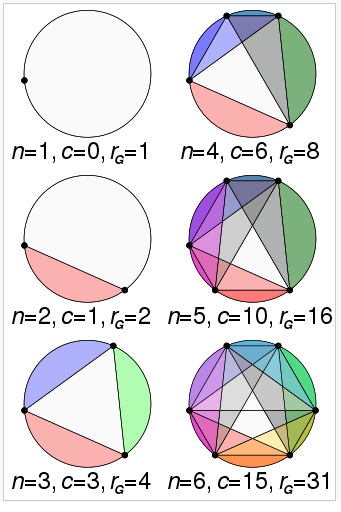
\includegraphics[scale=0.75]{images/strong_law_small_num.png}
\end{center}
 
Loosely, it states, “There aren’t enough small numbers to meet the many demands made of them.” Put another way, there are so many possible sequences generated in so many different ways that some of them will have to overlap for a while, even if they share no real connection with each other.
	
One of the most famous examples of this is the following function: Given a positive integer n, raise the number e (approximately $2.71828$) to the power of $(n – 1)/2$. Then, take the least integer above that number. As we do this for the first few positive integers, the numbers produced are $1, 2, 3, 5, 8, 13, 21, 34$, and $55$. Does this look familiar? These are precisely the numbers of the famed Fibonacci sequence! As it turns out, however, this magical Fibonacci generator fails after $55$: the next few terms are $91, 149,$ and $245$.

Another version of the Strong Law also shows up if you’ve ever had the fortune of hand-drawing complex geometry diagrams. Consider the following problem, which has recently made its way into mathematical lore:

Alice is practicing drawing triangles. She wants to draw an acute triangle whose angle measures are all multiples of $10$ (in degrees), is not isosceles, and has no $30-$ or $60-$ degree angles (to avoid some special coincidences). How many distinct triangles can Alice draw?
 
Taken one at a time, these are all very reasonable requests. But, if you do the working out, you’ll find that there are actually zero possible triangles that satisfy all of the criteria simultaneously! Alice is out of luck – a diagrammatic coincidence seems inevitable.

It’s important to note that while the Strong Law of Small Numbers is certainly present in many scenarios, it doesn’t reduce the power of conjecture and creativity in math. Sure, there are some seemingly-amazing patterns that chalk up to nothing more than a numerical coincidence. On the flip side, however, some of our greatest discoveries have also been uncovered via quantum leaps of faith. Just don’t jump to too many conclusions the next time you see a suspicious-looking pattern in a problem – as Guy puts it, “You can’t tell by looking.” 
\begin{center}
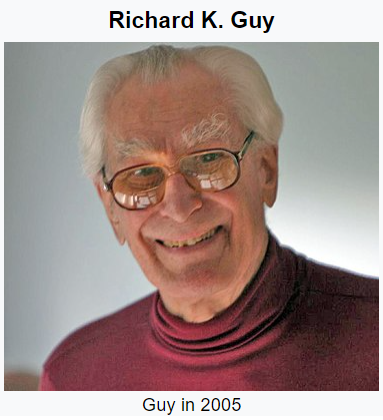
\includegraphics[scale=0.75]{images/richard_guy.png}
\end{center}
\end{document}